\section{Spanish Grand prix}

\subsection{Circuit Analysis}

\textbf{Circuit Name:} Circuit de Barcelona-Catalunya (Montmeló, Spain) \\
\textbf{Length:} 4.657 km - \textbf{Laps:} 66 - \textbf{Total Distance:} 307.236 km

\begin{figure}[H]
    \centering
    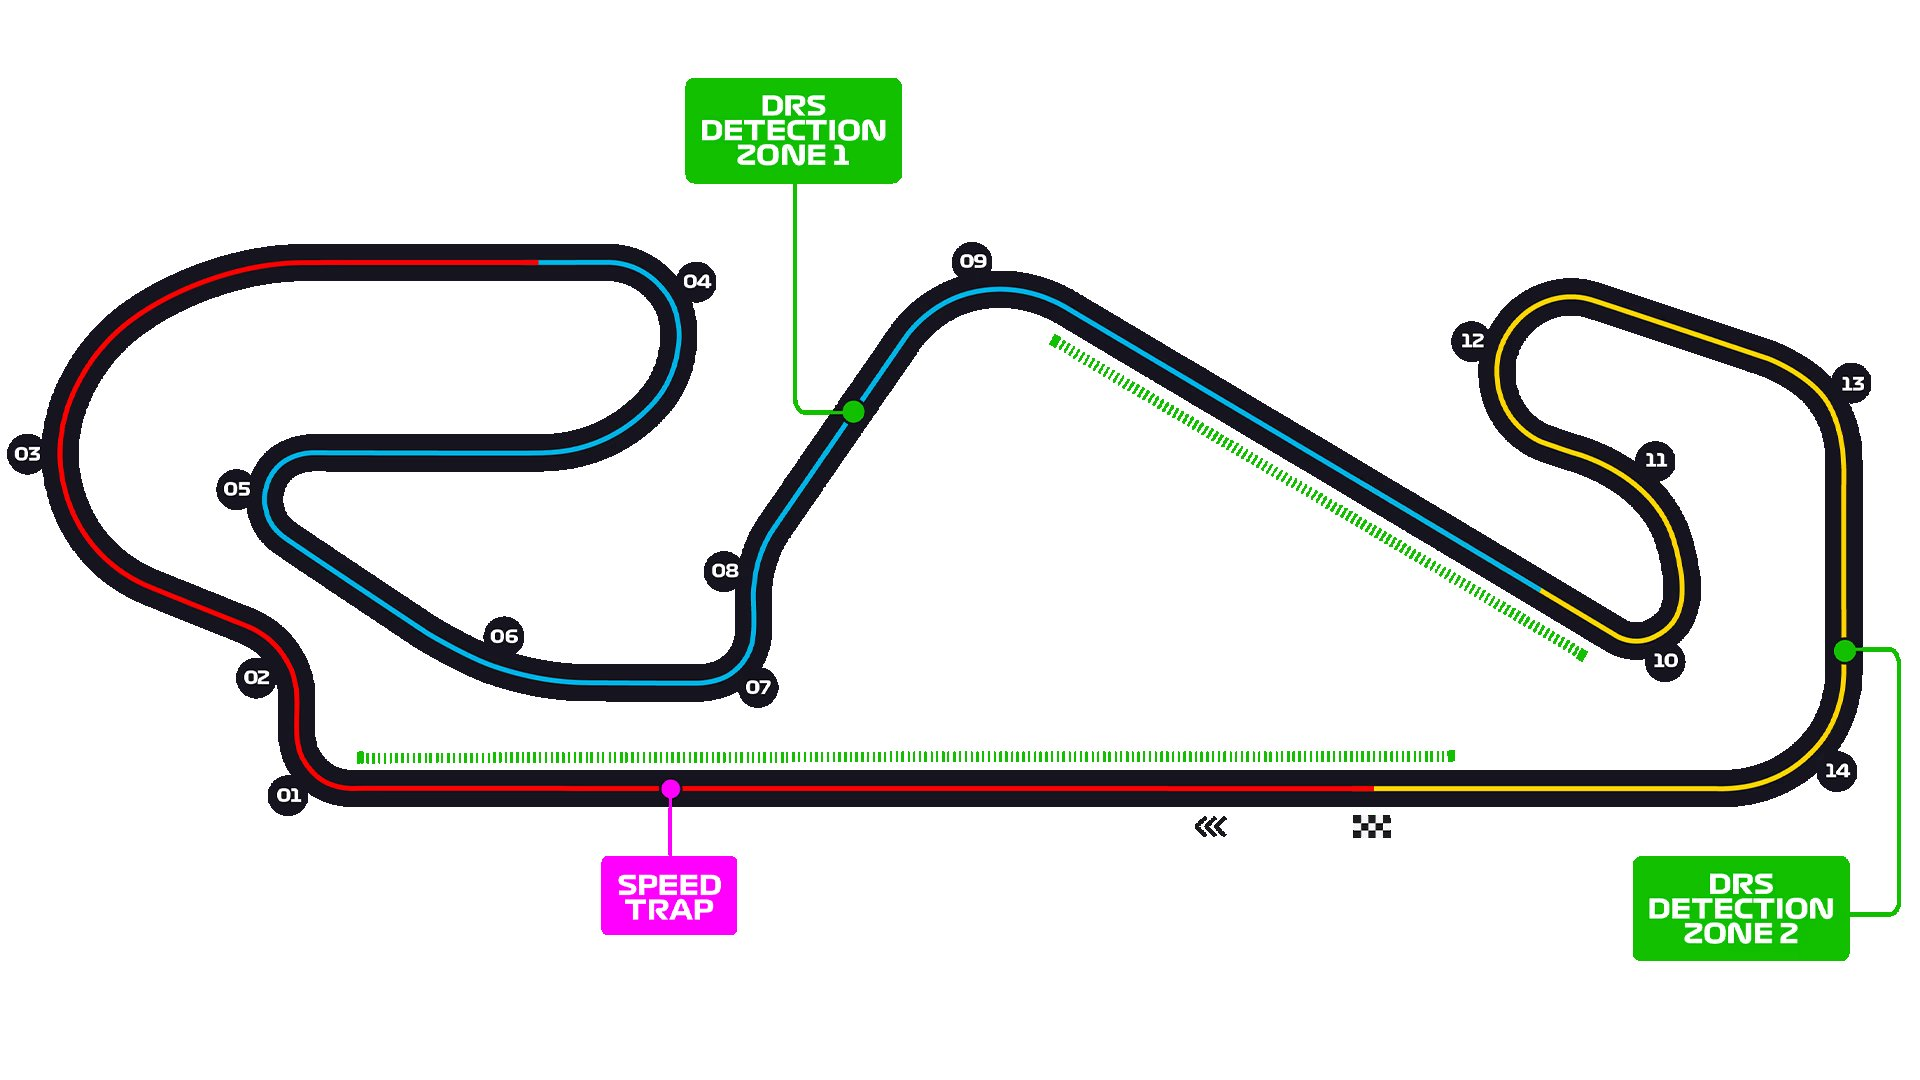
\includegraphics[width=0.75\linewidth]{images/10.Spain_Circuit.jpg}
\end{figure}

\begin{itemize}
    \item \textbf{Lap Record} : 1:12.272 (2023, Max Verstappen - Red Bull).
    
    \item \textbf{Number of Corners \& Key Features} : 14 turns (8 right, 6 left) - Known for its mix of high-, medium-, and low-speed corners, including long Turn 3 and quick Turn 9 (Campsa). Final sector technical, requiring high downforce.
    
    \item \textbf{Braking Zones \& Traction} : Heavy braking at Turn 1 (first chicane) and Turn 10 (La Caixa). Good traction needed out of the final corner onto the main straight.
    
    \item \textbf{DRS \& Overtaking} : Two DRS zones (main straight, between Turns 9–10).\\
    Best overtaking into Turn 1 and Turn 10, though turbulence still makes overtaking challenging.
    
    \item \textbf{Tyre Degradation \& Strategy} : Circuit is abrasive and demanding on tyres, especially front-left.\\
    Two-stop strategies are the norm, tyre management is crucial in hot Spanish conditions.
    
    \item \textbf{Weather \& Environment} : Typically hot and sunny in June, with track temps exceeding 40°C. Wind direction in Turn 3 and Turn 9 often impacts car stability.
\end{itemize}

\textbf{Strategic Summary :}
Barcelona tests overall car performance balance, aero efficiency, tyre management, and downforce. A benchmark track where the fastest car usually wins, but strategy execution remains key.


\subsection{Race Analysis}

\textbf{Date:} 23 June 2024 — 15:00 local time 

\begin{itemize}
    \item \textbf{Qualifying Summary} : \textbf{Pole Position:} Lando Norris (McLaren) – 1:11.383 (new track record). \\
    Grid: Verstappen 2nd, Hamilton 3rd, Russell 4th.\\
    Ferrari struggled for single-lap pace, starting behind Mercedes.
    
    \item \textbf{Race Summary} : \textbf{Winner:} Max Verstappen (Red Bull).\\
    \textbf{Podium:} 1. Verstappen - 2. Norris - 3. Hamilton.
    
    \item \textbf{Strategies} : Standard two-stop race (Medium–Hard–Medium or Medium–Medium–Hard).\\ 
     - Verstappen executed undercut perfectly on Norris at first stop. \\
     - Norris extended his first stint but couldn’t regain track position. \\
     - Mercedes split strategies, Hamilton’s tyre life gave podium edge. \\
     - Ferrari mirrored top strategies but lacked outright pace.\\
    
    \item \textbf{Performance Trends} : \textbf{Red Bull:} Verstappen not dominant by huge margin but managed lead with control. Pérez again underwhelming in P8. \\
    \textbf{McLaren:} Norris had the fastest car on track according to both drivers: pole, fastest lap, and P2 confirm pace. Piastri recovered to P7. \\
    \textbf{Mercedes:} Best race of 2024 so far. Hamilton returned to podium, Russell strong but beaten late. \\
    \textbf{Ferrari:} Solid but not a winning threat. Leclerc and Sainz P5–P6 after failing to match McLaren/Red Bull/Mercedes. \\
    \textbf{Alpine:} Back-to-back double points (Gasly P9, Ocon P10), confirming Montréal form.
    
    \item \textbf{Championship Impact} : \textbf{Drivers:} Verstappen 219 points, Norris 150 (+1), Leclerc 148 (-1).\\
    \textbf{Constructors:} Red Bull 330, Ferrari 270, McLaren 237, Mercedes 151.    
\end{itemize}

\textbf{Key Takeaway :}
Verstappen overturned Norris’s pole with strategic precision and tyre pace. McLaren continued to prove their competitiveness, while Mercedes showed steady recovery. Ferrari faded, marking a step back in the title fight.


\subsection{Link \& Takeaway}

\begin{itemize}
    \item Barcelona rewarded Red Bull’s superior tyre management and strategy execution, key to beating Norris. 
    \item McLaren’s strong qualifying and pace confirmed their rise, but track position loss at pit stops proved decisive. 
    \item Mercedes demonstrated progress with Hamilton’s podium, while Ferrari struggled with setup and consistency. 
    \item The race reinforced Barcelona’s status as a “benchmark” track, exposing the true pecking order.
\end{itemize}